\chapter{Testování}

Cílem testování v~této práci je zjistit výkonost jednotlivých platforem a~porovnat je vůči sobě. 

Testy jsou zaměřeny primárně na měření časů průběhu hlavní smyčky při určitých činnostech, tak aby bylo možné srovnat výkonost a~stabilitu jednotlivých platforem. 
Stabilitou je v~tomto případě myšlen rozdíl mezi minimálním a~maximálním naměřeným časem průchodu smyčky v~rámci opakovaných měření a~jednotlivých průchodů.

Při předchozí práci s~\EVthree{ } a~standardně dodávaným prostředím jsem v~rámci základního testování zjistil, že minimální perioda hlavní smyčky s~pár příkazy na vyčtení dat ze senzoru a následného nastavení motorů dle těchto hodnot (klasický program na jízdu po čáře) není kratší než 10~ms. 
Vzhledem k~výkonu procesoru (32-bitový ARM na 300~MHz) v~\EVthree{ }je tento čas velmi zarážející. 

O~to větší překvapení nastalo, když jsem srovnával průměrnou periodu s~maximální. Ukázalo se, že ačkoliv je průměrná perioda přibližně 20~ms, maximální perioda může dosahovat až~100~ms. 
Takto velký rozptyl je pro potřeby regulace velmi problematický. 
Ve většině případů je potřeba mít konstantní čas průchodu hlavní smyčkou, aby rozdíl v~časech periody neovlivňoval měření a~následné řízení. 

Pokud bude nutné zajistit stabilní periodu, je třeba softwarově zpomalit průběh hlavní smyčky na maximální naměřený čas. 
Jedině tak lze zajistit konstantní periodu. 
Když by se použil tento postup, dostali bychom se na frekvenci 10~Hz, což je z~pohledu regulace již velmi nepříznivá hodnota.

Tyto testy byly provedeny na velmi jednoduchém programu. 
V případě rozsáhlejších projektů, kde by se pracovalo s~více vlákny a~periferiemi mohou být výsledky ještě horší.

Proto jsem se rozhodl provést důkladné testování s~ekvivalentními programy na jednotlivých platformách a~zjistit, jestli tyto neduhy některá z~nich neodstraňuje a~za jakých situací k podobným problémům dochází.

\section{Forma testování}

Na počátku jsem zvažoval dvě formy testování. První počítala s~rozsáhlejší metodikou, v~rámci které bych testoval různé funkce \EVthree{}~\brick{{\it u}} a~zjišťoval, kde mohou být nejproblémovější místa z~pohledu výkonu. \\

V~rámci testů jsem se chtěl zaměřit na několik oblastí: % a jejich kombinace.

\begin{itemize}
	\item matematické operace
	\item čtení senzorů
	\item řízení motorů
	\item práce se soubory
	\item vícevláknové/procesové programy
\end{itemize}  

Druhá varianta měla zajistit co možná nejstejnoměrnější podmínky měření času tak, aby jej neovlivňovalo fungování jednotlivých platforem. 
Proto mělo být k měření využito Arduino Uno a~velmi jednoduchý program  (příklad programu ve standardním prostředí pro \EVthree{ }na obrázku \ref{fig:LoopTimeLEDblinking-measuring}).
Program by jen blikal s dvěma LED\footnote{LED = Light-Emitting Diode –- dioda emitující světlo} (zelenou a červenou) umístěnými na přední straně pod ovládacími tlačítky na \EVbrick{{\it u}} a~čas svitu jednotlivých LED by měřilo Arduino.

%U jednotlivých platforem by se měřili časy průchodů hlavní smyčkou a z těchto naměřených dat by se vytvářeli histogramy pro následné vyhodnocení.

% Následně jsem se ale rozhodl pro jinou strategii testování. 
% Rozhodl jsem se ale pro jinou strategii testování. 

% Po čase jsem tuto strategii zavrhl. 

Jednalo by se totiž o~jeden z~nejlepších způsobů, jak demostrovat problémy s~dobou trvání jednotlivých cyklů a~práci s periferiemi. 
V~optimálním případě by totiž mělo kombinací těchto dvou barevných LED vzniknout oranžová. 
Pokud by se tak nestalo, pozorovatel by měl hned optickou zpětnou vazbu a~zároveň lze jednoduše měřit časové prodlevy mezi spínáním a~vypínáním jednotlivých LED pomocí měřící sestavy s Arduinem.

\begin{figure}[h]
	\centering
	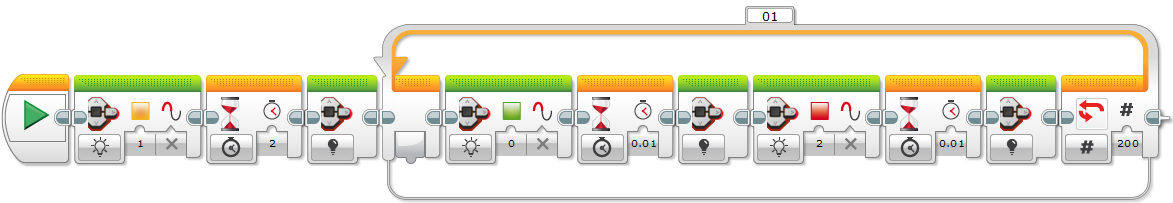
\includegraphics[width=\textwidth]{images/measuring-ev3-software_LoopTimeLEDblinking.png}
	\caption[Ukázka jednoduchého programu na blikání zelenou a červenou LED]{Ukázka jednoduchého programu na blikání zelenou a červenou LED}
	\label{fig:LoopTimeLEDblinking-measuring}
\end{figure}

Ukázkový program je připraven tak, že každá LED se vždy rozsvítí na 10~milisekund ($T~=~0.01~s~= 10~ms$), následně zhasne a~rozsvítí se druhá LED.  
Celkový čas jednoho průchodu cyklem trvá 20~ms ($T~=~T_{LED1}~+ T_{LED2}$) a~frekvence blikání by měla být 50~Hz ($f~=~\frac{1}{T}~= \frac{1}{0.02~s} =~50~Hz$). 
Což je frekvence, kterou již lidské oko nezaznamená (filmy mají standardní frekvenci obnovování snímku 24 až 30~Hz). % TODO: a běžné televizní vysílání má 50~Hz).
Celkový počet opakování hlavní smyčky je zvolen na 200. 
Blikání má tedy probíhat 4~sekundy ($t~=~T~\cdot~counter =~0.02~ms~\cdot~200~= 4~s$).

Pro měřící sestavu byl vybrán fototranzistor BPX~81\footnote{\url{http://cz.rs-online.com/web/p/fototranzistory/6655255/}} (má velmi široké rozpětí vstupních vlnových délek -- zvládne viditelné i~infra světlo) s~Arduinem Uno (viz obrázek~\ref{fig:arduino-measuring-system}). \\

Tato kombinace mi přijde nejvhodnější z~několika důvodů: 

\begin{itemize}
	\item velmi rozšířený hardware (Arduino Uno)
	\item rychlé sestavení
	\item možnost snadného naprogramování
	\item jednoduchá duplikovatelnost (zopakování experimentu)
\end{itemize}  

Nejdůležitějším bodem pro tuto variantu byla jednoduchá duplikovatelnost, která umožňuje komukoliv provést stejná měření, ať už pro kontrolu v~této práci prezentovaných výsledků nebo pro otestování jiné platformy a~porovnání s~naměřenými daty z~této práce.

\begin{figure}[h]
	\centering
	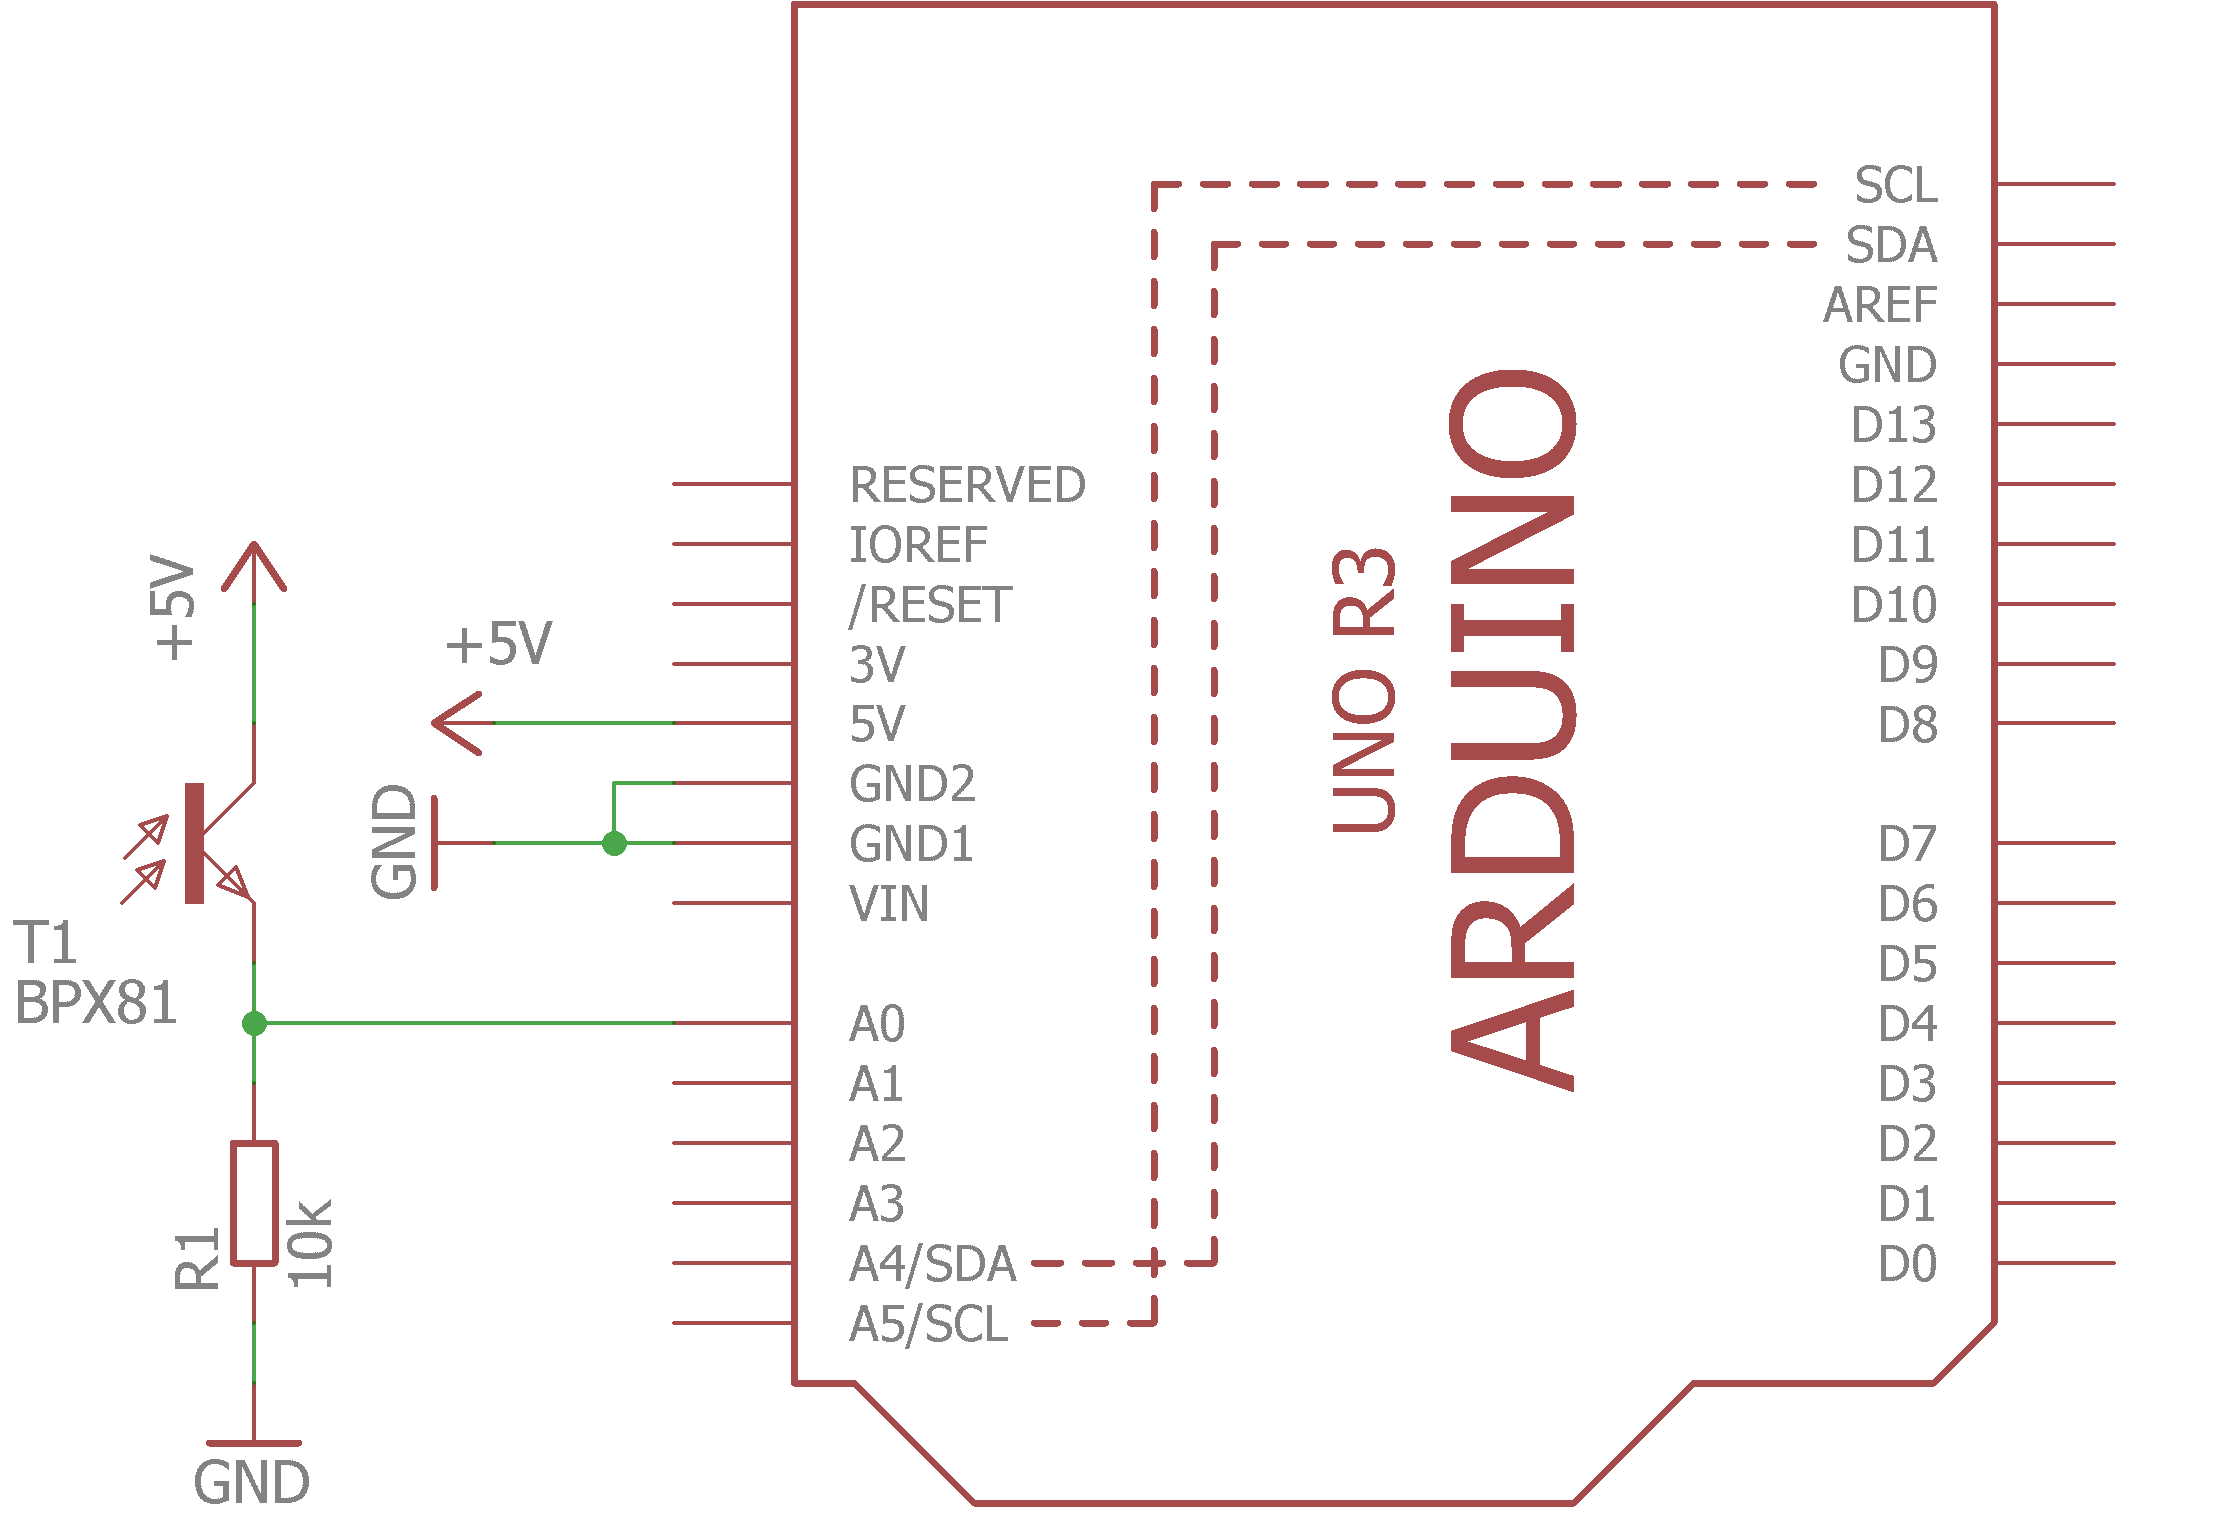
\includegraphics[width=250px]{images/measuring-arduino-system_schema.png}	
	\caption[Schema zapojení měřícího systému]{Schema zapojení měřícího systému}
	\label{fig:arduino-measuring-system}
\end{figure}

Jelikož se druhá varianta zdála vhodnější, otestoval jsem ji s~programem, prezentovaným výše, s~danou měřící sestavou a~osciloskopem. 

\begin{figure}[h]
	\centering
	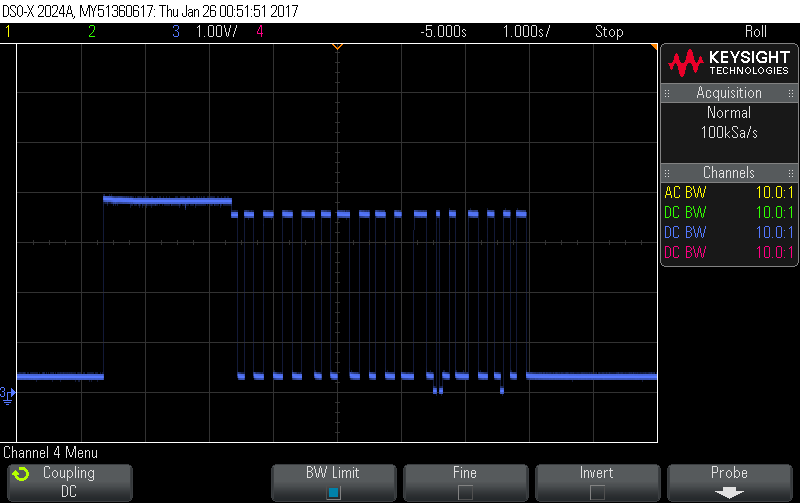
\includegraphics[width=350px]{images/measuring-oscilloscope_ev3-software_led-blinking_all.png}
	\caption[Záznam signálu z osciloskopu po provedení zkušebního programu]{Záznam signálu z osciloskopu po provedení zkušebního programu}
	\label{fig:measuring_lego-ev3_orig-soft_led-blinking_all}
\end{figure}

Výsledky byli velice překvapivé. Celkový počet pulzů červené LED (napětí na osciloskopu přibližně 3,7~V; pro zelenou 0,3~V; oranžová 3,9~V) byl 17 
(viz obrázek~\ref{fig:measuring_lego-ev3_orig-soft_led-blinking_all}). Přičemž dle programu mělo proběhnout 200~pulzů.  

Při detailním zkoumání se ukázalo, že LED nedokáží blikat na 50~Hz, ale mohou svůj stav měnit vždy s~frekvencí 20~Hz. 
Každých 50~ms docházelo ke kontrole stavových proměnných u~LED a~případné změně stavu (viz~obrázek~\ref{fig:measuring_lego-ev3_orig-soft_led-blinking_part1} -- jeden dílek odpovídá 100~ms a~1~V).

%Pravděpodobným vysvětlením tohoto chovaní je 

Toto chování lze například vysvětlit tak, že v~rámci operačního systému \EVbrick{\it u} je v určité periodě (přibližně 50~ms) vyvoláno přerušení od časovače, které porovná stav proměnných a~registrů LED a~dle výsledku buď rozsvítí nebo zhasne. 
Proto v~daných intervalech dochází k~interferenci mezi časováním LED (20~ms) a~interního přerušení (přibližně 50~ms) a~podle toho, jak se tyto události sejdou se jednotlivé LED přepínají.
Tento časovač bude pravděpodobně fungovat jen pro LED, ale nebude dále ovlivňovat další chování systému.
 
\begin{figure}[h]
	\centering
	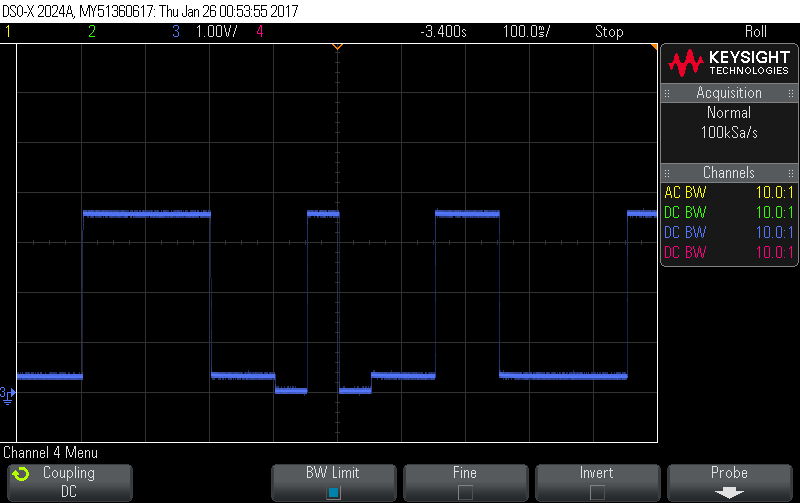
\includegraphics[width=350px]{images/measuring-oscilloscope_ev3-software_led-blinking_part1.png}
	\caption[Zoom na záznam z osciloskopu po provedení zkušebního programu]{Zoom na záznam z osciloskopu po provedení zkušebního programu}
	\label{fig:measuring_lego-ev3_orig-soft_led-blinking_part1}
\end{figure}

\begin{figure}[h]
	\centering
	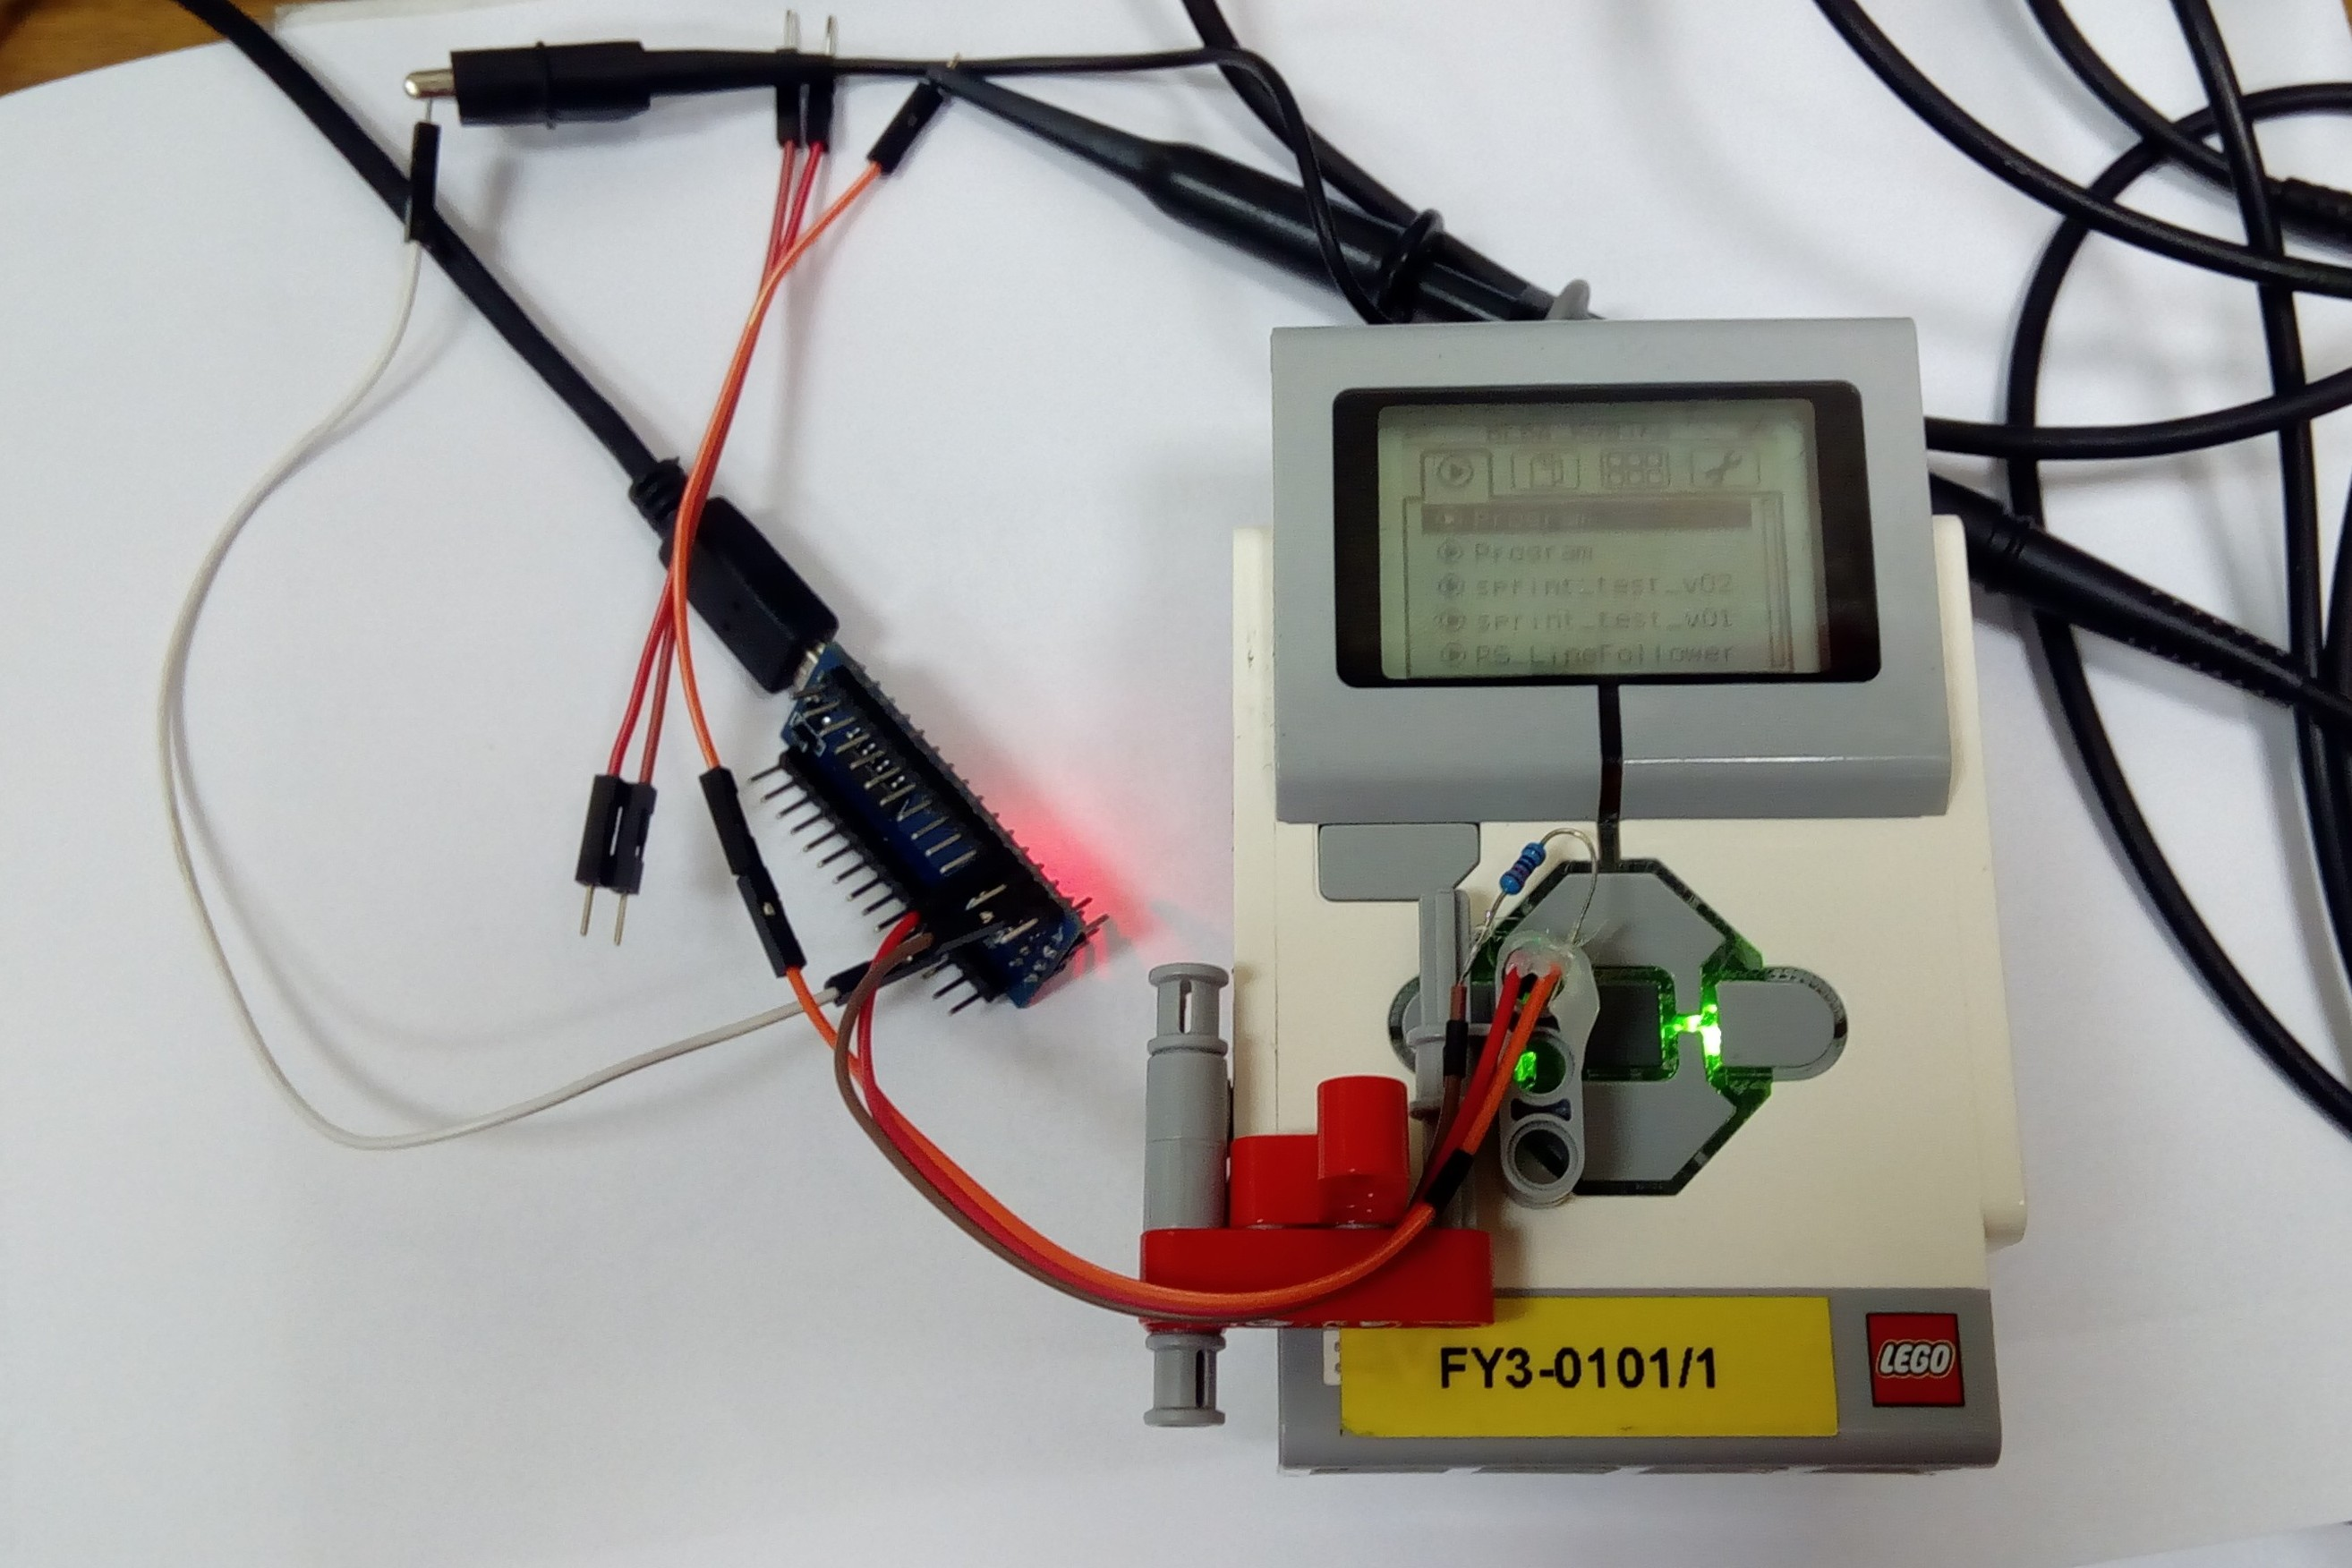
\includegraphics[width=280px]{images/measuring-system_photo.jpg}
	\caption[Foto měřící sestavy]{Foto měřící sestavy}
	\label{fig:measuring-system_photo}
\end{figure}

Z~naměřených výsledků vyplývá, že tuto formu testování nelze použít.
% a~bude potřeba nachystat rozsáhlejší testovací metodiku, pro obsluhu jednotlivých funkcí systémů a~platforem, jak je napsáno v úvodu této kapitoly.
Rozhodl jsem se tedy vyhodnotit jednotlivé systémy na základě uživatelského pocitu a mých zkušeností s jednotlivými systémy.

% TODO